\documentclass[a4paper, 12pt]{article}
\usepackage{bm}
\usepackage{amssymb}
\usepackage{graphicx}
\usepackage{amsmath}
\usepackage{amsfonts}
\usepackage{float}
\usepackage{wrapfig}
\graphicspath{ {images/} }
\begin{document}
\begin{center} 
{\Huge{\textbf{Instantons}}}\\
\end{center}

\section {What are Instantons?}
Instantons refer to localised finite-action solutions of the classical Euclidean field equations of a theory. They are in some sense similar to solitons but instead they are localised in time. 
\section {How to get Euclidean action?}
To go from Minkowsi space to Euclidean space we do the analytic continuation of time, i.e. t$\to -i\tau$, this is also called \textbf{Wick rotation}. The Euclidean action is defined as
\begin{equation}
S_{Euc} = -i(S_{Min})_{continued}
\end{equation}
As an example let's see the Minkowski Klien-Gordon system. The action is 
\begin{equation}
S_{Min} = \int dt \int dx \bigg[\frac{1}{2}\bigg(\frac{\partial\phi}{\partial t} \bigg)^2 - \frac{1}{2}(\nabla \phi)^2 -m^2 \phi^2  \bigg],
\end{equation}
which yields the field equation
\begin{equation}
\bigg( \frac{\partial^2}{\partial t^2} - \nabla^2 \bigg)\phi + m^2\phi = 0.
\end{equation}
So doing the processes mentioned above, we get that
\begin{equation}
S_{Min} = \int dx_4 \int dx \bigg[\frac{1}{2}\bigg(\frac{\partial\phi}{\partial x_4} \bigg)^2 + \frac{1}{2}(\nabla \phi)^2 + m^2 \phi^2  \bigg]
\end{equation}
which yields the field equation
\begin{equation}
\bigg( \frac{\partial^2}{\partial {x_4}^2} + \nabla^2 \bigg)\phi - m^2\phi = 0.
\end{equation}
Since we can write the path integral as
\begin{equation}
G(q_i,q_f;t) = \int Dq \*\ \textrm{exp}\bigg[\frac{i}{\hbar}S_{Min}\bigg] =  \int Dq \*\ \textrm{exp}\bigg[\frac{i}{\hbar}\int_0^t dt \bigg(\frac{m}{2}\dot{q^2} - V(q) \bigg) \bigg]
\end{equation}
In the imaginary time we can also write this as
\begin{equation}
G_E(q_i,q_f;\tau) = \int Dq \*\ \textrm{exp}\bigg[-\frac{1}{\hbar}S_{Euc}\bigg] =  \int Dq \*\ \textrm{exp}\bigg[\frac{i}{\hbar}\int_0^\tau d\tau' \bigg(\frac{m}{2}\dot{q^2} + V(q) \bigg) \bigg].
\end{equation}
One can see that the potential V becomes -V. We can see the same thing from the stationary phase equations
\begin{equation}
-m\ddot{q} + V'(q) = 0.
\end{equation}

Some important observations:
\begin{itemize}
\item Minkowski energy $\equiv$ Euclidean action.
\item The Euclidean action is like static soliton solutions in higher dimensions.
\item  Like the finiteness of energy of solitons, here we have finiteness of Euclidean action. From the path-integral representation we can see that if action is infinite it leads to zero contribution.
\end{itemize}


Before looking into the instanton problem we first need to see the semiclassics from the path integral.


\section {Semiclassics from path integral}

The general functional integral we have is of the form $\int Dx $ $e^{-F[x]}$. We use the stationary phase approximation and do the taylor series expansion of the functional. To get the stationary path we minimize the functional and get the classical path.
\begin{equation}
\frac{\delta F[x]}{\delta x(t)} \Bigg|_{x=\bar{x}} = 0.
\end{equation}
Now we Taylor expand the functional to second order around $\bar{x}$, i.e.
\begin{equation}
F[x] = F[\bar{x}+y] = F[\bar{x}] + \frac{1}{2}\int dt \int dt' y(t')A(t,t')y(t) + ... ,
\end{equation}
where $A(t,t') = \frac{\delta^2 F[x]}{\delta x(t) \delta x(t')} \bigg|_{x=\bar{x}}$ denotes the second functional derivative.\\
If the operator $\hat{A} \equiv \{A(t,t')\}$ is positive definite, then the functional integration reduces to
\begin{equation}
\int Dx \*\ e^{-F[x]} \simeq e^{-F[\bar{x}]} \textrm{det}\bigg(\frac{\hat{A}}{2\pi}\bigg)^{-1/2}.
\end{equation}
Putting the lagrangian as $L(q,\dot{q}) = m\dot{q}^2/2 - V(q)$, we get the second functional derivative as:
\begin{equation}
 \frac{1}{2}\int dt \int dt' r(t')A(t,t')r(t) =  -\frac{1}{2}\int dt  r(t')[m\partial^2_t + V''(q_{cl})]r(t).
\end{equation}
As an example of the above let's see a quantum particle in a well. Let the well be centred around $q=0$. Let's evaluate G(0,0;t), minimising the action gives the classical path as $q_{cl}(t)=0$ whoch then further gives $S[q_{cl}(t)]=0$. On expanding the potential we get, $V''(q)= m\omega^2$. This gives the transition amplitude as
\begin{equation}
G(0,0;t) \simeq \int Dr \*\ \textrm{exp} \bigg[-\frac{i}{\hbar}\int_0^t dt'  r(t')\frac{m}{2}(\partial^2_{t'} + \omega^2)]r(t')\bigg].
\end{equation}
This integral gives us
\begin{equation}
G(0,0;t) \simeq J \textrm{det}(-m(\partial^2_{t} + \omega^2)/2)^{-1/2}
\end{equation}
Finding the eigenvalues and then evaluating the determinant gives us
\begin{equation}
G(0,0;t) \simeq J \sqrt{\frac{m\omega}{2\pi i \hbar \textrm{sin}(\omega t)}} \*\ \Theta(t).
\end{equation}
The above expression is exact for harmonic oscillator. We will now use this tool to evaluate the double well potential.

\section {Double well potential: tunneling and instantons}
\begin{figure}[ht]
    \centering
    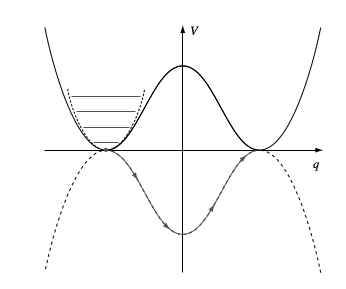
\includegraphics[height=5cm, width=6cm]{fig1}
\end{figure}










\begin{figure}[ht]
    \centering
    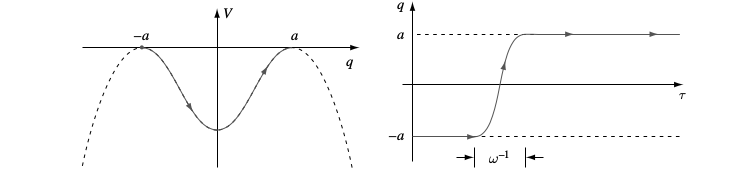
\includegraphics[height=4cm, width=15cm]{fig2}
\end{figure}
\begin{figure}[ht]
    \centering
    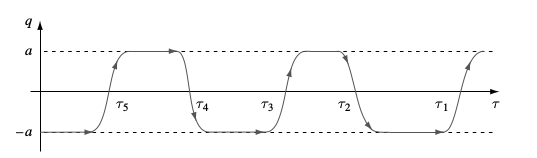
\includegraphics[height=4cm, width=15cm]{fig3}
\end{figure}
\begin{figure}[ht]
    \centering
    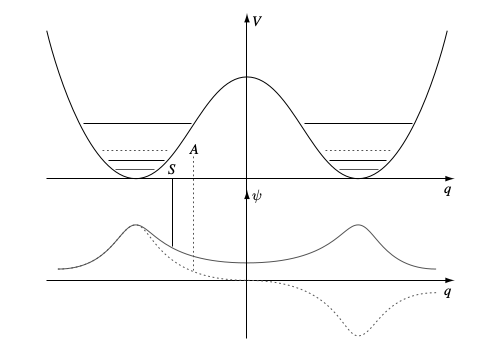
\includegraphics[height=5cm, width=8cm]{fig4}
\end{figure}






\section {Escape from metastable minimum: bounces}
\begin{figure}[ht]
    \centering
    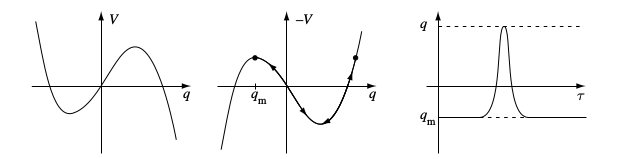
\includegraphics[height=4cm, width=15cm]{fig5}
\end{figure}
If we want to calculate the survival probability, the probability amplitude of remaining at the potential minimum $q_m$.


\section {Tunneling of quantum fields}

\begin{figure}[ht]
    \centering
    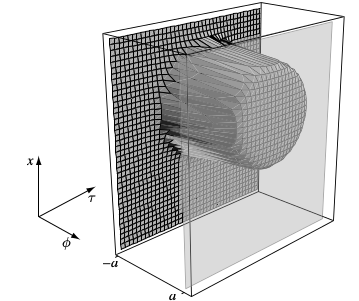
\includegraphics[height=9cm, width=9cm]{fig6}
\end{figure}







\end{document}